\begin{figure*}[!t]
\vspace{-0.5ex}
\centering
  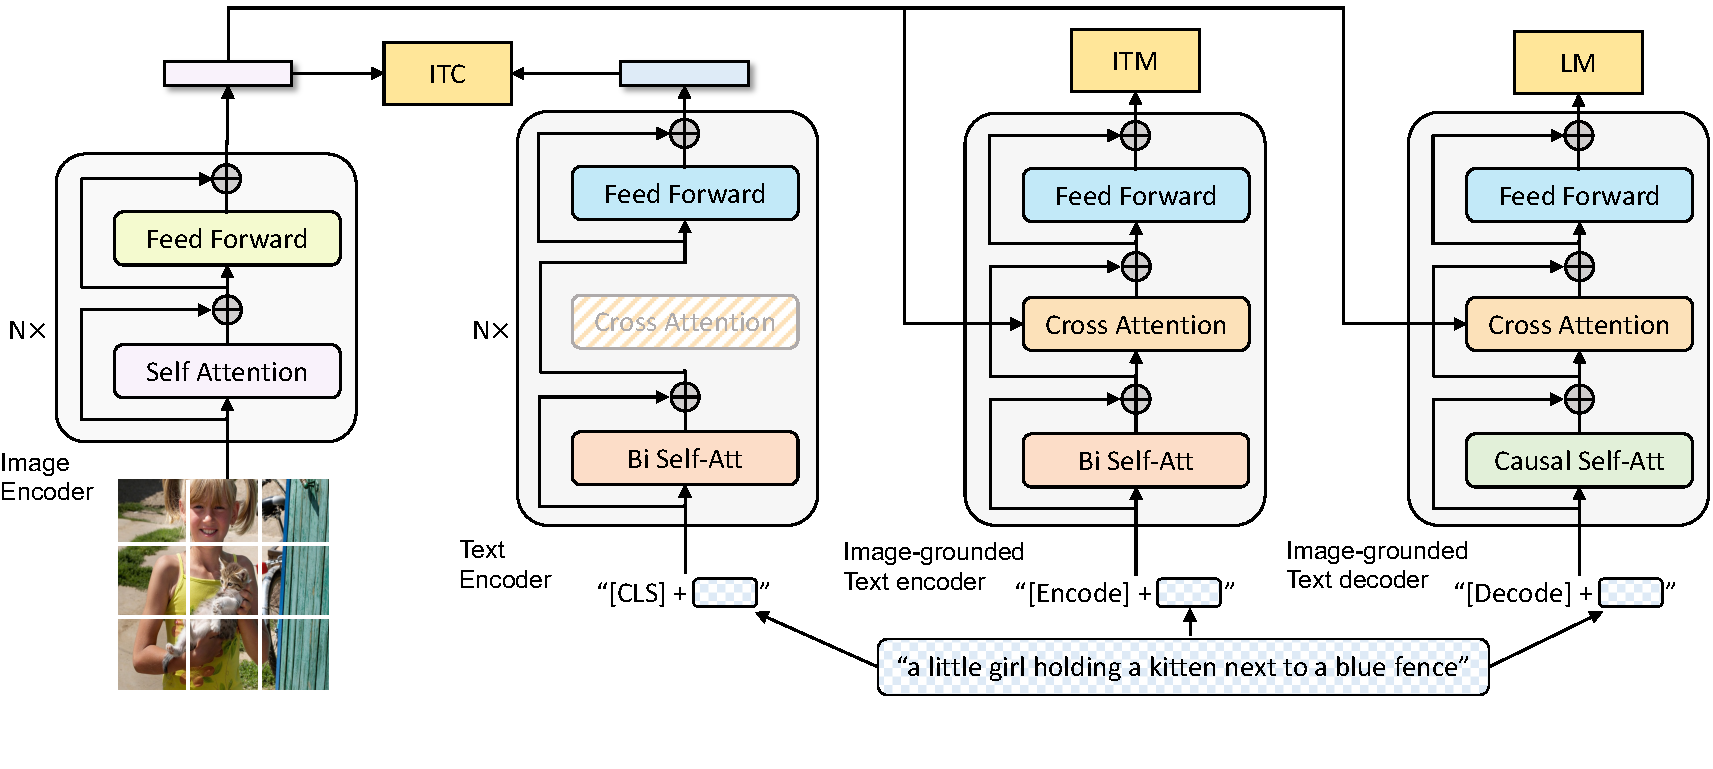
\includegraphics[width=0.98\textwidth]{imgs/MED.pdf}
\vspace{-6ex}
\caption{Pre-training model architecture and objectives of \name~(same parameters have the same color). We propose multimodal mixture of encoder-decoder, a unified vision-language model which can operate in one of the three functionalities:
(1) Unimodal encoder is trained with an image-text contrastive (ITC) loss to align the vision and language representations.
(2) Image-grounded text encoder uses additional cross-attention layers to model vision-language interactions,
and is trained with a image-text matching (ITM) loss to distinguish between positive and negative image-text pairs.
(3) Image-grounded text decoder replaces the bi-directional self-attention layers with causal self-attention layers,
and shares the same cross-attention layers and feed forward networks as the encoder. The decoder is trained with a language modeling (LM) loss to generate captions given images. 
}
\vspace{-2ex}
\label{fig:med}
\end{figure*}
